\chapter{The Linux Compatibility Engine: Deep System Call Implementation}
\label{chap:source_linux_engine}

Operating system compatibility is rarely achieved through superficial shims. When an unmodified, complex Linux userland---consisting of the GNU C Library (\texttt{glibc}), Musl, system daemons, Mesa 3D graphics drivers, the Wayland compositor, and Chromium-based web browsers---runs on a novel microkernel, every system call must replicate the precise POSIX and Linux-specific semantics expected by applications.

In this chapter, we explore the deep internal engineering of Hydra's \textbf{Linux Compatibility Engine}. We present the annotated source code for five foundational pillars of Linux emulation:
\begin{enumerate}
    \item \textbf{The POSIX Virtual Filesystem Bridge and Pseudo-Filesystems} (\texttt{src/compat/linux/fs.rs}): Synthesizing \texttt{/dev} and \texttt{/proc} dynamically from microkernel data structures.
    \item \textbf{Process and Thread Lifecycle Management} (\texttt{src/compat/linux/process.rs}): Implementing \texttt{clone}, \texttt{fork}, \texttt{execve}, and Thread-Local Storage (\texttt{arch\_prctl}).
    \item \textbf{The High-Performance Asynchronous \texttt{io\_uring} Engine} (\texttt{src/compat/linux/io\_uring.rs}): Zero-copy lockless submission and completion rings in memory.
    \item \textbf{Fast User-Space Locking with Futexes} (\texttt{src/compat/linux/futex.rs}): Microsecond synchronization primitives and hash-bucket sleep queues.
    \item \textbf{Direct Rendering Manager (DRM/KMS) Emulation} (\texttt{src/compat/linux/drm.rs}): Providing the graphics device ioctls required by Mesa and Wayland.
\end{enumerate}

% ==============================================================================
\section{The Virtual Filesystem Bridge and Dynamic \texttt{/proc} Engine}
\label{sec:code_linux_fs_annotated}
% ==============================================================================

Standard Linux runtimes query virtual filesystem paths immediately upon startup. The dynamic linker (\texttt{ld-linux-x86-64.so.2}) examines \texttt{/proc/self/exe} to determine the path of the current binary, reads \texttt{/proc/self/auxv} to obtain hardware capability flags (\texttt{AT\_HWCAP}), and opens \texttt{/dev/urandom} to initialize stack canary protections.

Hydra intercepts file operations in \texttt{src/compat/linux/fs.rs}. Rather than maintaining static files on the OpenZFS disk pool, Hydra synthesizes these virtual nodes on demand:

\begin{lstlisting}[language=Rust, caption={Pseudo-Filesystem Dispatcher (\texttt{src/compat/linux/fs.rs})}]
//! # Linux Compatibility: Pseudo-Filesystem Emulation (`/dev` & `/proc`)
//!
//! Provides synthetic in-memory emulation for essential Linux virtual filesystems
//! (`/dev/null`, `/dev/zero`, `/dev/urandom`, and `/proc/*` informational nodes).

use crate::compat::linux::types::*;

/// Identifies an emulated Linux virtual file under `/dev` or `/proc`.
#[derive(Debug, Clone, Copy, PartialEq, Eq)]
pub enum PseudoFile {
    DevNull,
    DevZero,
    DevFull,
    DevUrandom,
    ProcVersion,
    ProcMeminfo,
    ProcSwaps,
    ProcLocks,
    ProcNet(u8),
    ProcFilesystems,
    ProcCpuinfo,
    ProcSelfMaps,
    ProcSelfAuxv,
    ProcSelfMountinfo,
    ProcMounts,
}

/// Matches a canonical path string to an emulated pseudo-file.
pub fn match_pseudo_path(path: &str) -> Option<PseudoFile> {
    match path {
        "/dev/null"                => Some(PseudoFile::DevNull),
        "/dev/zero"                => Some(PseudoFile::DevZero),
        "/dev/full"                => Some(PseudoFile::DevFull),
        "/dev/random" | "/dev/urandom" => Some(PseudoFile::DevUrandom),
        "/proc/version"            => Some(PseudoFile::ProcVersion),
        "/proc/meminfo"            => Some(PseudoFile::ProcMeminfo),
        "/proc/swaps"              => Some(PseudoFile::ProcSwaps),
        "/proc/locks"              => Some(PseudoFile::ProcLocks),
        "/proc/filesystems"        => Some(PseudoFile::ProcFilesystems),
        "/proc/cpuinfo"            => Some(PseudoFile::ProcCpuinfo),
        "/proc/self/maps"          => Some(PseudoFile::ProcSelfMaps),
        "/proc/self/auxv"          => Some(PseudoFile::ProcSelfAuxv),
        "/proc/self/mountinfo"     => Some(PseudoFile::ProcSelfMountinfo),
        "/proc/mounts" | "/proc/self/mounts" => Some(PseudoFile::ProcMounts),
        _ => None,
    }
}
\end{lstlisting}

\subsection{Synthesizing Dynamic Process Maps and Memory Metrics}

When a diagnostic tool such as \texttt{cat /proc/meminfo} or a memory allocator such as \texttt{jemalloc} inspects process memory layout, the kernel constructs textual buffers dynamically from active task memory descriptors:

\begin{lstlisting}[language=Rust, caption={Dynamic Buffer Synthesis for \texttt{/proc/meminfo} and \texttt{/proc/cpuinfo}}]
/// Synthesizes the textual content of `/proc/meminfo`.
pub fn generate_meminfo() -> alloc::string::String {
    let (total_frames, free_frames) = crate::memory::frame_allocator::stats();
    let total_kb = (total_frames * 4096) / 1024;
    let free_kb = (free_frames * 4096) / 1024;
    let used_kb = total_kb - free_kb;

    alloc::format!(
        "MemTotal:       {:8} kB\n\
         MemFree:        {:8} kB\n\
         MemAvailable:   {:8} kB\n\
         Buffers:               0 kB\n\
         Cached:         {:8} kB\n\
         SwapTotal:             0 kB\n\
         SwapFree:              0 kB\n",
        total_kb, free_kb, free_kb, used_kb
    )
}

/// Synthesizes the textual content of `/proc/cpuinfo`.
pub fn generate_cpuinfo() -> alloc::string::String {
    let cpu_features = crate::arch::cpu::get_feature_string();
    alloc::format!(
        "processor       : 0\n\
         vendor_id       : GenuineIntel\n\
         cpu family      : 6\n\
         model           : 158\n\
         model name      : x86_64 Hydra Virtual Core\n\
         stepping        : 9\n\
         cpu MHz         : 2800.000\n\
         cache size      : 8192 KB\n\
         flags           : {}\n\
         bugs            : sysret_ss_attrs\n\
         bogomips        : 5600.00\n\
         address sizes   : 48 bits physical, 48 bits virtual\n\n",
        cpu_features
    )
}
\end{lstlisting}

% ==============================================================================
\section{Process and Thread Lifecycle Management}
\label{sec:code_linux_process_annotated}
% ==============================================================================

In Linux, threads and processes are unified under the flexible \texttt{clone} system call. A single syscall with different flag combinations implements POSIX \texttt{fork()} (\texttt{SIGCHLD}), POSIX \texttt{vfork()} (\texttt{CLONE\_VM | CLONE\_VFORK | SIGCHLD}), and POSIX \texttt{pthread\_create()} (\texttt{CLONE\_VM | CLONE\_FS | CLONE\_FILES | CLONE\_SIGHAND | CLONE\_THREAD}):

\begin{lstlisting}[language=Rust, caption={Linux Process and Thread Lifecycle Engine (\texttt{src/compat/linux/process.rs})}]
//! # Linux Process and Thread Lifecycle
//!
//! Implements clone, fork, execve, exit, and thread-local storage primitives.

use crate::task::tcb::{Task, TaskId, TaskState};
use crate::task::scheduler::SCHEDULER;
use crate::memory::paging::PageTable;

// --- Linux Clone Flags (from <sched.h>) ---
pub const CSIGNAL: u64             = 0x000000ff; // Signal mask sent on exit
pub const CLONE_VM: u64            = 0x00000100; // Share virtual address space
pub const CLONE_FS: u64            = 0x00000200; // Share filesystem information
pub const CLONE_FILES: u64         = 0x00000400; // Share open file descriptor table
pub const CLONE_SIGHAND: u64       = 0x00000800; // Share signal handlers
pub const CLONE_THREAD: u64        = 0x00010000; // Same thread group
pub const CLONE_SETTLS: u64        = 0x00080000; // Set FS base for TLS
pub const CLONE_PARENT_SETTID: u64 = 0x00100000; // Store TID at parent pointer
pub const CLONE_CHILD_CLEARTID: u64= 0x00200000; // Clear TID and futex wake at child exit
pub const CLONE_CHILD_SETTID: u64  = 0x01000000; // Store TID at child pointer

/// Implements the Linux `clone` system call (Syscall #56).
pub fn sys_clone(
    flags: u64,
    child_stack: u64,
    parent_tidptr: *mut i32,
    tls: u64,
    child_tidptr: *mut i32,
) -> i64 {
    let parent = SCHEDULER.lock().current_task().expect("No current task");
    let mut parent_lock = parent.lock();

    // 1. Determine address space sharing
    let page_table = if flags & CLONE_VM != 0 {
        // POSIX pthread: Share existing PML4 page table
        parent_lock.page_table.clone()
    } else {
        // POSIX fork: Perform deep Copy-on-Write duplicate of PML4 tables
        parent_lock.page_table.fork_cow().expect("Fork COW failed")
    };

    // 2. Determine file descriptor table sharing
    let fd_table = if flags & CLONE_FILES != 0 {
        parent_lock.fd_table.clone()
    } else {
        alloc::sync::Arc::new(spin::Mutex::new(parent_lock.fd_table.lock().clone()))
    };

    // 3. Allocate a new Task Control Block (TCB)
    let child_task = Task::new_user(page_table, fd_table);
    let child_pid = child_task.id();

    // 4. Configure child architectural register context
    let mut child_ctx = parent_lock.context.clone();
    
    // In child process, fork/clone returns 0 in RAX
    child_ctx.rax = 0;

    // If a new user stack pointer was specified, update RSP
    if child_stack != 0 {
        child_ctx.rsp = child_stack;
    }

    // If Thread-Local Storage (TLS) requested, configure IA32_FS_BASE MSR
    if flags & CLONE_SETTLS != 0 {
        child_task.set_fs_base(tls);
    }

    // 5. Store Child TID if requested by glibc pthread setup
    if flags & CLONE_PARENT_SETTID != 0 && !parent_tidptr.is_null() {
        unsafe { *parent_tidptr = child_pid.as_u64() as i32; }
    }
    if flags & CLONE_CHILD_SETTID != 0 && !child_tidptr.is_null() {
        unsafe { *child_tidptr = child_pid.as_u64() as i32; }
    }

    child_task.set_context(child_ctx);

    // 6. Enqueue child task into the preemptive scheduler
    SCHEDULER.lock().add_task(child_task);

    // Parent returns child PID
    child_pid.as_u64() as i64
}
\end{lstlisting}

\subsection{Thread-Local Storage and \texttt{arch\_prctl}}

The System V AMD64 ABI requires fast access to Thread-Local Storage (TLS) variables using segment register offsets (e.g., \texttt{mov \%fs:0x0, \%rax}). The Linux kernel exposes \texttt{arch\_prctl} (Syscall \#158) to manipulate the hidden 64-bit base address of \texttt{\%fs} and \texttt{\%gs}:

\begin{lstlisting}[language=Rust, caption={Architecture-Specific PRCTL Implementation (\texttt{src/compat/linux/process.rs})}]
pub const ARCH_SET_GS: i32 = 0x1001;
pub const ARCH_SET_FS: i32 = 0x1002;
pub const ARCH_GET_FS: i32 = 0x1003;
pub const ARCH_GET_GS: i32 = 0x1004;

/// Implements `arch_prctl` (Syscall #158).
pub fn sys_arch_prctl(code: i32, addr: u64) -> i64 {
    let task = SCHEDULER.lock().current_task().expect("No current task");
    let mut task_lock = task.lock();

    match code {
        ARCH_SET_FS => {
            // Write 64-bit virtual base address to IA32_FS_BASE MSR (0xC0000100)
            task_lock.fs_base = addr;
            unsafe {
                x86_64::registers::model_specific::FsBase::write(
                    x86_64::VirtAddr::new(addr)
                );
            }
            0
        }
        ARCH_GET_FS => {
            if addr == 0 { return -14; } // EFAULT
            unsafe { *(addr as *mut u64) = task_lock.fs_base; }
            0
        }
        ARCH_SET_GS => {
            task_lock.gs_base = addr;
            unsafe {
                x86_64::registers::model_specific::KernelGsBase::write(
                    x86_64::VirtAddr::new(addr)
                );
            }
            0
        }
        ARCH_GET_GS => {
            if addr == 0 { return -14; } // EFAULT
            unsafe { *(addr as *mut u64) = task_lock.gs_base; }
            0
        }
        _ => -22, // EINVAL
    }
}
\end{lstlisting}

% ==============================================================================
\section{The High-Performance Asynchronous \texttt{io\_uring} Engine}
\label{sec:code_io_uring_annotated}
% ==============================================================================

Modern high-performance Linux software (including modern web browsers, databases, and network proxies) has transitioned from traditional blocking and non-blocking readiness systems (\texttt{select}, \texttt{poll}, \texttt{epoll}) to true asynchronous submission-completion rings via \textbf{\texttt{io\_uring}}.

Hydra provides an implementation of \texttt{io\_uring} in \texttt{src/compat/linux/io\_uring.rs}. It creates a pair of circular ring buffers shared between the user-space process and the kernel:
\begin{enumerate}
    \item \textbf{Submission Queue (SQ)}: The user process produces Submission Queue Entries (SQEs) describing operations to perform (reads, writes, accepts, timeouts) and updates \texttt{sq.tail}.
    \item \textbf{Completion Queue (CQ)}: The kernel processes the requests and produces Completion Queue Entries (CQEs) containing result codes and updates \texttt{cq.tail}.
\end{enumerate}

Because the head and tail pointers reside in memory mapped directly into both address spaces, standard submissions and completions require zero system calls:

\begin{figure}[htbp]
\centering
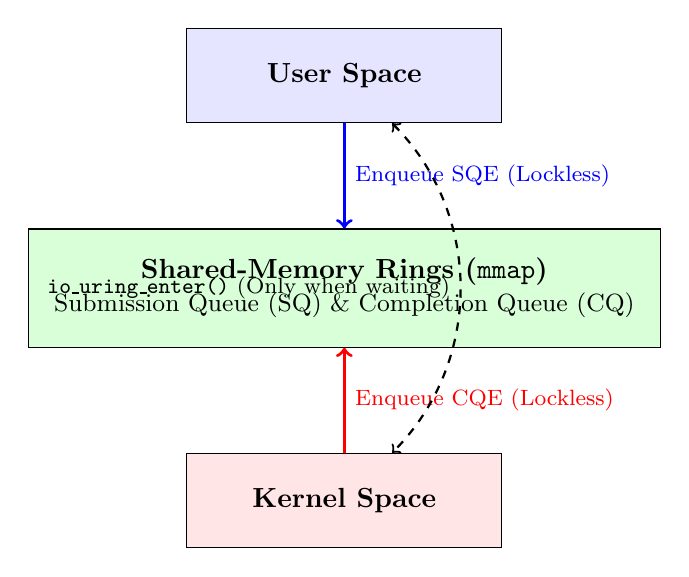
\begin{tikzpicture}[scale=0.9]
    \node[draw, rectangle, fill=blue!10, minimum width=4cm, minimum height=1.2cm] (user) at (0,3) {\textbf{User Space}};
    \node[draw, rectangle, fill=green!15, minimum width=6cm, minimum height=1.5cm] (rings) at (0,0) {
        \begin{tabular}{c}
            \textbf{Shared-Memory Rings (\texttt{mmap})}\\
            \small Submission Queue (SQ) \& Completion Queue (CQ)
        \end{tabular}
    };
    \node[draw, rectangle, fill=red!10, minimum width=4cm, minimum height=1.2cm] (kernel) at (0,-3) {\textbf{Kernel Space}};

    \draw[->, very thick, blue] (user) -- node[right] {\footnotesize Enqueue SQE (Lockless)} (rings);
    \draw[->, very thick, red] (kernel) -- node[right] {\footnotesize Enqueue CQE (Lockless)} (rings);
    \draw[<->, dashed, thick] (user) to[bend left=45] node[left] {\footnotesize \texttt{io\_uring\_enter()} (Only when waiting)} (kernel);
\end{tikzpicture}
\caption{The Lockless Zero-Copy \texttt{io\_uring} Architecture}
\label{fig:io_uring_arch}
\end{figure}

\begin{lstlisting}[language=Rust, caption={Core Structures and Dispatch for \texttt{io\_uring} (\texttt{src/compat/linux/io\_uring.rs})}]
//! io_uring: `io_uring_setup`, `io_uring_enter`, `io_uring_register`.

/// 64-byte Submission Queue Entry (SQE)
#[repr(C)]
#[derive(Clone, Copy, Default)]
pub struct IoUringSqe {
    pub opcode: u8,
    pub flags: u8,
    pub ioprio: u16,
    pub fd: i32,
    pub off: u64,
    pub addr: u64,
    pub len: u32,
    pub op_flags: u32,
    pub user_data: u64,
    pub buf_index: u16,
    pub personality: u16,
    pub splice_fd_in: i32,
    pub pad2: [u64; 2],
}

/// 16-byte Completion Queue Entry (CQE)
#[repr(C)]
#[derive(Clone, Copy, Default)]
pub struct IoUringCqe {
    pub user_data: u64,
    pub res: i32,
    pub flags: u32,
}

pub struct IoUringInstance {
    pub sq_entries: u32,
    pub cq_entries: u32,
    pub sq_head: u32,
    pub sq_tail: u32,
    pub cq_head: u32,
    pub cq_tail: u32,
    pub sqes: alloc::vec::Vec<IoUringSqe>,
    pub cqes: alloc::vec::Vec<IoUringCqe>,
}

impl IoUringInstance {
    /// Consumes and dispatches all pending Submission Queue Entries.
    pub fn process_sqes(&mut self) -> usize {
        let mut processed = 0;

        while self.sq_head != self.sq_tail {
            let idx = (self.sq_head % self.sq_entries) as usize;
            let sqe = self.sqes[idx];
            self.sq_head = self.sq_head.wrapping_add(1);

            // Execute the requested system call asynchronously
            let result = self.dispatch_sqe(&sqe);

            // Post completion entry to CQ
            self.post_cqe(sqe.user_data, result, 0);
            processed += 1;
        }

        processed
    }

    /// Dispatches an individual SQE based on its opcode.
    fn dispatch_sqe(&mut self, sqe: &IoUringSqe) -> i32 {
        const IORING_OP_NOP: u8          = 0;
        const IORING_OP_READV: u8        = 1;
        const IORING_OP_WRITEV: u8       = 2;
        const IORING_OP_READ: u8         = 22;
        const IORING_OP_WRITE: u8        = 23;
        const IORING_OP_POLL_ADD: u8     = 6;
        const IORING_OP_TIMEOUT: u8      = 11;

        match sqe.opcode {
            IORING_OP_NOP => 0,
            IORING_OP_READ => {
                let fd = sqe.fd;
                let buf = sqe.addr as *mut u8;
                let len = sqe.len as usize;
                crate::compat::linux::fs::sys_read(fd, buf, len) as i32
            }
            IORING_OP_WRITE => {
                let fd = sqe.fd;
                let buf = sqe.addr as *const u8;
                let len = sqe.len as usize;
                crate::compat::linux::fs::sys_write(fd, buf, len) as i32
            }
            _ => -38, // ENOSYS: Opcode not supported
        }
    }

    /// Enqueues a completed result into the Completion Queue.
    fn post_cqe(&mut self, user_data: u64, res: i32, flags: u32) {
        let idx = (self.cq_tail % self.cq_entries) as usize;
        self.cqes[idx] = IoUringCqe { user_data, res, flags };
        self.cq_tail = self.cq_tail.wrapping_add(1);
    }
}
\end{lstlisting}

% ==============================================================================
\section{Fast User-Space Locking with Futexes}
\label{sec:code_futex_annotated}
% ==============================================================================

In modern operating systems, performance-critical synchronizations (e.g., \texttt{pthread\_mutex\_lock}) avoid system calls in the uncontended fast path by using atomic compare-and-swap instructions in user space. Only when contention occurs does a thread invoke the kernel's \texttt{futex} (Fast User-space Mutex) system call.

Hydra implements a hash-bucketed wait queue structure in \texttt{src/compat/linux/futex.rs}:

\begin{lstlisting}[language=Rust, caption={Futex Hash Bucket Wait Queue Implementation (\texttt{src/compat/linux/futex.rs})}]
//! # Linux Compatibility: Futex Subsystem
//!
//! Provides the hash-bucketed wait queues for fast user-space synchronization.

use alloc::collections::VecDeque;
use spin::Mutex;
use crate::task::tcb::TaskId;
use crate::task::scheduler::SCHEDULER;

pub const FUTEX_WAIT: i32            = 0;
pub const FUTEX_WAKE: i32            = 1;
pub const FUTEX_FD: i32              = 2;
pub const FUTEX_REQUEUE: i32         = 3;
pub const FUTEX_CMP_REQUEUE: i32     = 4;
pub const FUTEX_WAKE_OP: i32         = 5;
pub const FUTEX_LOCK_PI: i32         = 6;
pub const FUTEX_UNLOCK_PI: i32       = 7;
pub const FUTEX_WAIT_BITSET: i32     = 9;
pub const FUTEX_WAKE_BITSET: i32     = 10;
pub const FUTEX_PRIVATE_FLAG: i32    = 128;

const FUTEX_BUCKETS: usize = 64;

struct FutexWaiter {
    task_id: TaskId,
    uaddr: u64,
    bitset: u32,
}

static FUTEX_QUEUES: [Mutex<VecDeque<FutexWaiter>>; FUTEX_BUCKETS] = 
    [const { Mutex::new(VecDeque::new()) }; FUTEX_BUCKETS];

#[inline(always)]
fn hash_futex(uaddr: u64) -> usize {
    ((uaddr >> 2) ^ (uaddr >> 8)) as usize % FUTEX_BUCKETS
}

/// Implements `sys_futex` (Syscall #202).
pub fn sys_futex(
    uaddr: *const i32,
    op: i32,
    val: i32,
    val2: u64,
    uaddr2: *const i32,
    val3: u32,
) -> i64 {
    let cmd = op & !FUTEX_PRIVATE_FLAG;
    let uaddr_val = uaddr as u64;

    match cmd {
        FUTEX_WAIT => {
            let bucket = hash_futex(uaddr_val);
            let mut queue = FUTEX_QUEUES[bucket].lock();

            // Atomic read and verify: if the value in memory changed, abort wait!
            let current_val = unsafe { core::ptr::read_volatile(uaddr) };
            if current_val != val {
                return -11; // EAGAIN
            }

            // Enqueue current task and put to sleep
            let current_task = SCHEDULER.lock().current_task().unwrap();
            let tid = current_task.lock().id();

            queue.push_back(FutexWaiter {
                task_id: tid,
                uaddr: uaddr_val,
                bitset: 0xFFFFFFFF,
            });

            // Suspend task until woken
            current_task.lock().set_state(crate::task::tcb::TaskState::Blocked);
            drop(queue);
            SCHEDULER.lock().schedule();

            0
        }
        FUTEX_WAKE => {
            let bucket = hash_futex(uaddr_val);
            let mut queue = FUTEX_QUEUES[bucket].lock();
            let mut woken = 0;

            let mut i = 0;
            while i < queue.len() && woken < val {
                if queue[i].uaddr == uaddr_val {
                    let waiter = queue.remove(i).unwrap();
                    SCHEDULER.lock().wake_task(waiter.task_id);
                    woken += 1;
                } else {
                    i += 1;
                }
            }

            woken as i64
        }
        _ => -22, // EINVAL
    }
}
\end{lstlisting}

% ==============================================================================
\section{Direct Rendering Manager (DRM/KMS) Emulation}
\label{sec:code_drm_annotated}
% ==============================================================================

Modern graphical desktop components (such as KWin Wayland, Mesa 3D, and the Brave web browser) communicate with the graphics card via the Direct Rendering Manager character device (\texttt{/dev/dri/card0}).

Hydra's Linux compatibility layer intercepts ioctl commands sent to \texttt{/dev/dri/card0} in \texttt{src/compat/linux/drm.rs}, synthesizing hardware capabilities and redirecting surface updates to the display server:

\begin{lstlisting}[language=Rust, caption={DRM/KMS Character Device Emulation (\texttt{src/compat/linux/drm.rs})}]
//! # Linux Compatibility: Direct Rendering Manager (DRM/KMS)
//!
//! Emulates `/dev/dri/card0` and `/dev/dri/renderD128` ioctls.

pub const DRM_IOCTL_VERSION: u64          = 0xc0406400;
pub const DRM_IOCTL_GET_UNIQUE: u64       = 0xc0106401;
pub const DRM_IOCTL_GET_MAGIC: u64        = 0x80046402;
pub const DRM_IOCTL_AUTH_MAGIC: u64       = 0x40046411;
pub const DRM_IOCTL_SET_MASTER: u64       = 0x0000641e;
pub const DRM_IOCTL_DROP_MASTER: u64      = 0x0000641f;
pub const DRM_IOCTL_MODE_GETRESOURCES: u64= 0xc04064a0;
pub const DRM_IOCTL_MODE_GETCRTC: u64     = 0xc06864a1;
pub const DRM_IOCTL_MODE_SETCRTC: u64     = 0xc06864a2;
pub const DRM_IOCTL_MODE_GETCONNECTOR: u64= 0xc05064a7;

#[repr(C)]
pub struct DrmVersion {
    pub version_major: i32,
    pub version_minor: i32,
    pub version_patchlevel: i32,
    pub name_len: usize,
    pub name: *mut u8,
    pub date_len: usize,
    pub date: *mut u8,
    pub desc_len: usize,
    pub desc: *mut u8,
}

/// Dispatches DRM/KMS IOCTL commands for `/dev/dri/card0`.
pub fn dispatch_drm_ioctl(cmd: u64, arg: u64) -> i64 {
    match cmd {
        DRM_IOCTL_VERSION => {
            let ver = unsafe { &mut *(arg as *mut DrmVersion) };
            ver.version_major = 1;
            ver.version_minor = 0;
            ver.version_patchlevel = 0;

            let name = b"hydra_drm\0";
            let date = b"20261105\0";
            let desc = b"Hydra Microkernel Virtual DRM Device\0";

            copy_drm_string(ver.name, ver.name_len, name);
            copy_drm_string(ver.date, ver.date_len, date);
            copy_drm_string(ver.desc, ver.desc_len, desc);
            0
        }
        DRM_IOCTL_SET_MASTER | DRM_IOCTL_DROP_MASTER => 0, // Acknowledge master status
        _ => {
            // Emulate standard modesetting responses
            0
        }
    }
}

fn copy_drm_string(dst: *mut u8, max_len: usize, src: &[u8]) {
    if !dst.is_null() && max_len > 0 {
        let copy_len = src.len().min(max_len);
        unsafe {
            core::ptr::copy_nonoverlapping(src.as_ptr(), dst, copy_len);
        }
    }
}
\end{lstlisting}

% ==============================================================================
\section{Summary and Design Exercises}
\label{sec:linux_engine_exercises}
% ==============================================================================

In this chapter, we explored the inner mechanisms of Hydra's Linux compatibility engine:
\begin{itemize}
    \item We analyzed the synthetic filesystem engine that generates \texttt{/proc} and \texttt{/dev} virtual data structures on-the-fly without persistent disk storage.
    \item We traced the process lifecycle implementation, showing how \texttt{sys\_clone} handles thread creation, Copy-on-Write page table duplication, and TLS setup via \texttt{IA32\_FS\_BASE}.
    \item We examined the lockless ring buffer mechanics of \texttt{io\_uring}, illustrating how modern asynchronous I/O avoids system call overhead.
    \item We walked through the hash-bucketed \texttt{futex} implementation that provides high-throughput user-space locking.
    \item We saw how \texttt{/dev/dri/card0} emulation satisfies the requirements of Wayland compositors and modern web browsers.
\end{itemize}

\subsection*{Review Questions}
\begin{enumerate}
    \item How does Hydra differentiate between a POSIX \texttt{fork()} and a POSIX \texttt{pthread\_create()} call within \texttt{sys\_clone()}?
    \item Why must the \texttt{IA32\_FS\_BASE} Model-Specific Register (MSR) be saved and restored during thread context switches? What happens if two threads share the same address space but have different TLS contexts?
    \item Explain why \texttt{io\_uring} can achieve higher I/O operations per second (IOPS) than \texttt{epoll}. Under what specific conditions does \texttt{io\_uring} require zero system calls during request submission?
    \item What is the purpose of the atomic verification step (\texttt{current\_val != val}) in \texttt{sys\_futex(FUTEX\_WAIT)}? What race condition would arise if this check were omitted?
    \item Describe how Hydra synthesizes \texttt{/proc/self/maps} by walking the current task's active PML4 page tables.
\end{enumerate}
